\documentclass{article}

\usepackage{arxiv}

\usepackage[utf8]{inputenc} % allow utf-8 input
\usepackage[T1]{fontenc}    % use 8-bit T1 fonts
\usepackage{hyperref}       % hyperlinks
\usepackage{url}            % simple URL typesetting
\usepackage{booktabs}       % professional-quality tables
\usepackage{amsmath}
\usepackage{amsfonts}       % blackboard math symbols
\usepackage{nicefrac}       % compact symbols for 1/2, etc.
\usepackage{microtype}      % microtypography
\usepackage{cleveref}       % smart cross-referencing
\usepackage{lipsum}         % Can be removed after putting your text content
\usepackage{graphicx}
\usepackage{natbib}
\usepackage{doi}

\title{Audio classification with complex neural networks}

% Here you can change the date presented in the paper title
%\date{September 9, 1985}
% Or remove it
%\date{}

\author{Nikita Trufanov \\
	Bauman Moscow State Technical University\\
	2 Baumanskaya Street, Moscow, 105005, Russian Federation \\
	\texttt{trufanov@bmstu.ru} \\
	%% examples of more authors
	\And
	\href{https://orcid.org/0000-0001-5968-9883}{
\includegraphics[scale=0.06]{orcid.pdf}\hspace{1mm}Ivan Chernenkiy} \\
	I.M. Sechenov First Moscow State Medical University\\
	8-2 Trubetskaya str. Moscow, 119991, Russian Federation \\
	\texttt{chernenkiy\_i\_m@staff.sechenov.ru} \\
	\And
	\href{https://orcid.org/0000-0002-7651-3422}{
\includegraphics[scale=0.06]{orcid.pdf}\hspace{1mm}Oleg Kravchenko} \\
	Bauman Moscow State Technical University\\
	2 Baumanskaya Street, Moscow, 105005, Russian Federation \\
	\texttt{ok@bmstu.ru} \\
	\And
	\href{https://orcid.org/0000-0003-1891-4487}{
\includegraphics[scale=0.06]{orcid.pdf}\hspace{1mm}Dobroslav Egorov} \\
	Kotel’nikov Institute of Radioengineering and Electronics of Russian Academy of Sciences\\
	Mokhovaya st. 11-7, Moscow, 125009, Russian Federation \\
	\texttt{dobrix95@gmail.com} \\
}

% Uncomment to override  the `A preprint' in the header
%\renewcommand{\headeright}{Technical Report}
\renewcommand{\undertitle}{Technical Report}
% \renewcommand{\shorttitle}{\textit{arXiv} Template}

%%% Add PDF metadata to help others organize their library
%%% Once the PDF is generated, you can check the metadata with
%%% $ pdfinfo template.pdf
\hypersetup{
pdftitle={A template for the arxiv style},
pdfsubject={q-bio.NC, q-bio.QM},
pdfauthor={Nikita Trufanov, Ivan Chernenkiy, Oleg Kravchenko, Dobroslav Egorov},
pdfkeywords={phase spectrum, DFT, classification, complex-valued neural networks, audio, timbre},
}

\begin{document}
\maketitle

\begin{abstract}
In the vast majority of existing models for audio analysis, including those based on machine learning, only the amplitude-frequency representation of the original 
audio signals is involved, while the information which can be obtained from their phase spectrum is not taken into account. It is generally accepted that our 
auditory system is not sensitive to phase changes. However, starting with simple experiments on waveforms, one can come to a clear understanding that the phase
is quite important in terms of human perception of sound (especially low-pitched). So, for example, a change in the phase of some spectral components may lead
to a change in the audible pitch. If overtones can be distinguished in the spectrum, then a change in the phase relationships between these overtones may 
significantly affect the timbre of the sound. The phase shift of individual groups of overtones can lead to the appearance of an additional virtual pitch (f.e. church bell), 
and so on. All these effects are closely related to the phenomenon of dispersion during the wave propagation in physical media. It becomes clear that for deeper and intellectual 
audio analysis, the phase information is desirable to be taken into account and to be included as the input data of analytical models. Speaking of machine learning methods, 
particularly neural networks, most of them use real–valued numbers in computations for training and making inferences. Such models provide arguably the simplest input data 
representation: concatenation of the amplitude and phase offset parameters into a real–valued vector for further processing. But a more natural and at the same time elegant 
solution here seems to be the use of complex numbers and, accordingly, the so-called complex neural networks, which gain popularity in the machine learning community. 
Combining amplitude and phase information may be a missed opportunity to improve the quality of audio and speech signal processing. This paper aims to show that such 
complex–valued models are at least competitive with their real–valued counterparts. The performance of complex–valued neural networks for some speech and noise 
classification tasks is considered.
\end{abstract}


% keywords can be removed
\keywords{phase spectrum \and DFT \and classification \and complex-valued neural networks \and audio \and timbre }


\section{Introduction}
Signal processing for audio tasks such as classification [], segmentation [], filtering [],transcripting [] widely uses deep learning approaches. 
Current popularity of deep learning technique takes from 2012 for image classification task \citep{NIPS2012_c399862d}. 
Unlike images, audio is time series data with variable length. 
In this work we concentrated on sound event recognition (SER) task. Goal is to identify sounds occurring in everyday life. SER becoming key part in 
applications related to smart assistants \citep{cances2018sound}, healthcare \citep{kim2020occupant,khlaifi2018swallowing} or noise monitoring 
in industry \citet{Trufanov2021a}. 
Sound events are more random, both periodic and aperiodic, with less well-defined occurrence patterns. Sound events also exhibit much wider frequency and amplitude ranges. 
In last decade research community investigates usage of complex representation. It seeks for easier optimization and better generalization. In this work, 
we investigating usage of complex convolutions can better extract patterns from original data. 


\section{Complex-valued blocks}
\label{sec:headings}

\subsection{Complex convolution}
Complex convolution is operation of convolving complex filter matrix $\textbf{W}=\textbf{A}+i\textbf{B}$ 
with complex input data $\textbf{h}=\textbf{x}+i\textbf{y}$
 where $\textbf{A},\textbf{B},\textbf{x},\textbf{y}$ – real-valued and $i=\sqrt{-1}$. Convolution is defined as follows:
\begin{equation}
	f\left(\textbf{h}\right)=\textbf{W}\ast\textbf{h}=\left(\textbf{A}\ast\textbf{x}-\textbf{B}\ast\textbf{y}\right)+i(\textbf{B}\ast\textbf{x}+\textbf{A}\ast\textbf{y})
\end{equation}

\subsection{Complex Activation}
In real-valued neural networks widespread usage of ReLU-like family. Reasons are simple differentiation and implementation. In complex neural networks community numerous activations has been purposed.
 In our work we tested Complex ReLU(cReLU)\citet{Trabelsi2017} and zReLU\citep{guberman2016complex}. cReLU applied two separate ReLUs on both real and imaginary part of a neuron:
 \begin{equation}
	cReLU\left(z\right)=ReLU\left(Re\left(z\right)\right)+iReLU(Im(z))
\end{equation}
And zReLU is defined as:
\begin{equation}
	zReLU(z)=
	\begin{cases} 
		z & \text{if $\theta \in [0,\pi/2]$}\\
		0 & \text{otherwise}
	\end{cases}
\end{equation}


\section{Experiments}
\label{sec:experiments}
In our work we using CNN14 architecture \citep{Kong2019} as baseline for real. As framework we use 
PyTorch\citep{NEURIPS2019_9015}. For input it uses spectrogram features of 1 second duration at 
16000 sample rate. Each second selected randomly for each sample. 
It contains of 6 convolutional blocks and two linear layers. Each block consists of two 
convolutional layers, two batch normalizations and ReLU activations.

\begin{figure}
	\centering
	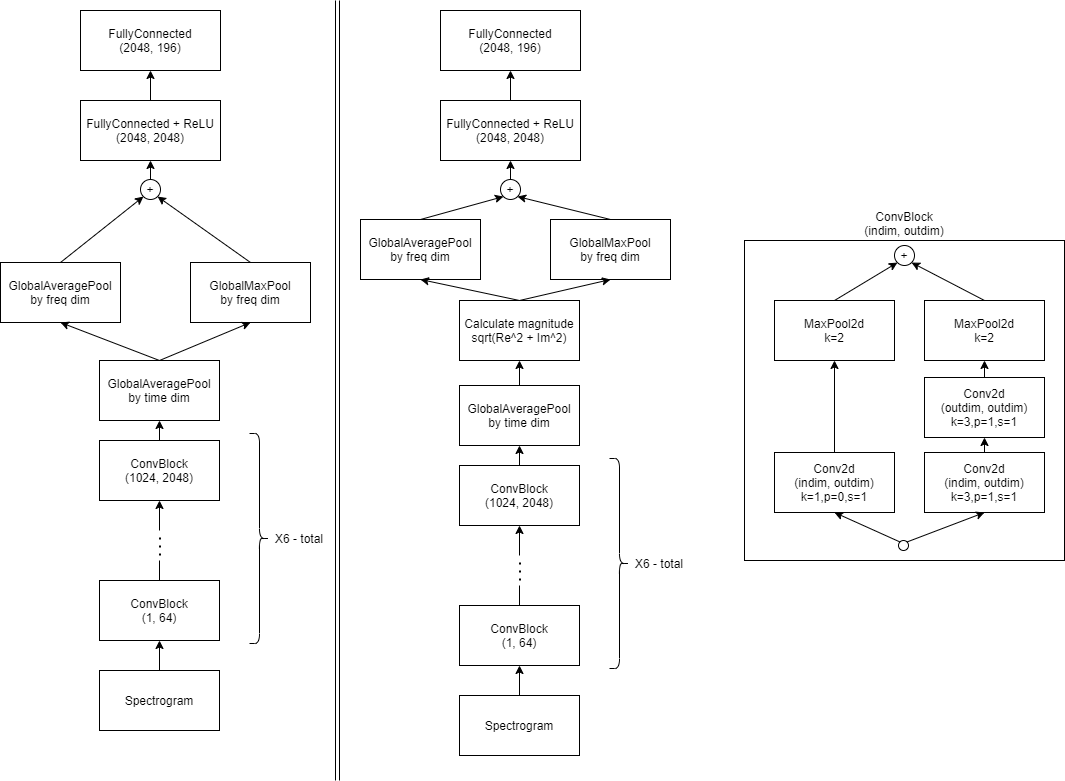
\includegraphics[width=0.49\linewidth]{assets/arch.png}
	\caption{Tested Architectures. On left side is real-valued version. On right side is complex-valued version}
	\label{fig:architectures}
\end{figure}

For complex counterpart we designed similar architecture. It also contains of 6 convolutional blocks 
and two linear layers. Each block does not have batch normalizations. In our work we found that usage of 
complex batch normalizations \citep{Trabelsi2017} do not help to converge at all. We will continue investigate
 this effect in our future. As activation function we used Complex ReLU\citep{Trabelsi2017}. As input we use complex spectrogram

\section{Results}

\begin{figure}
	\centering
	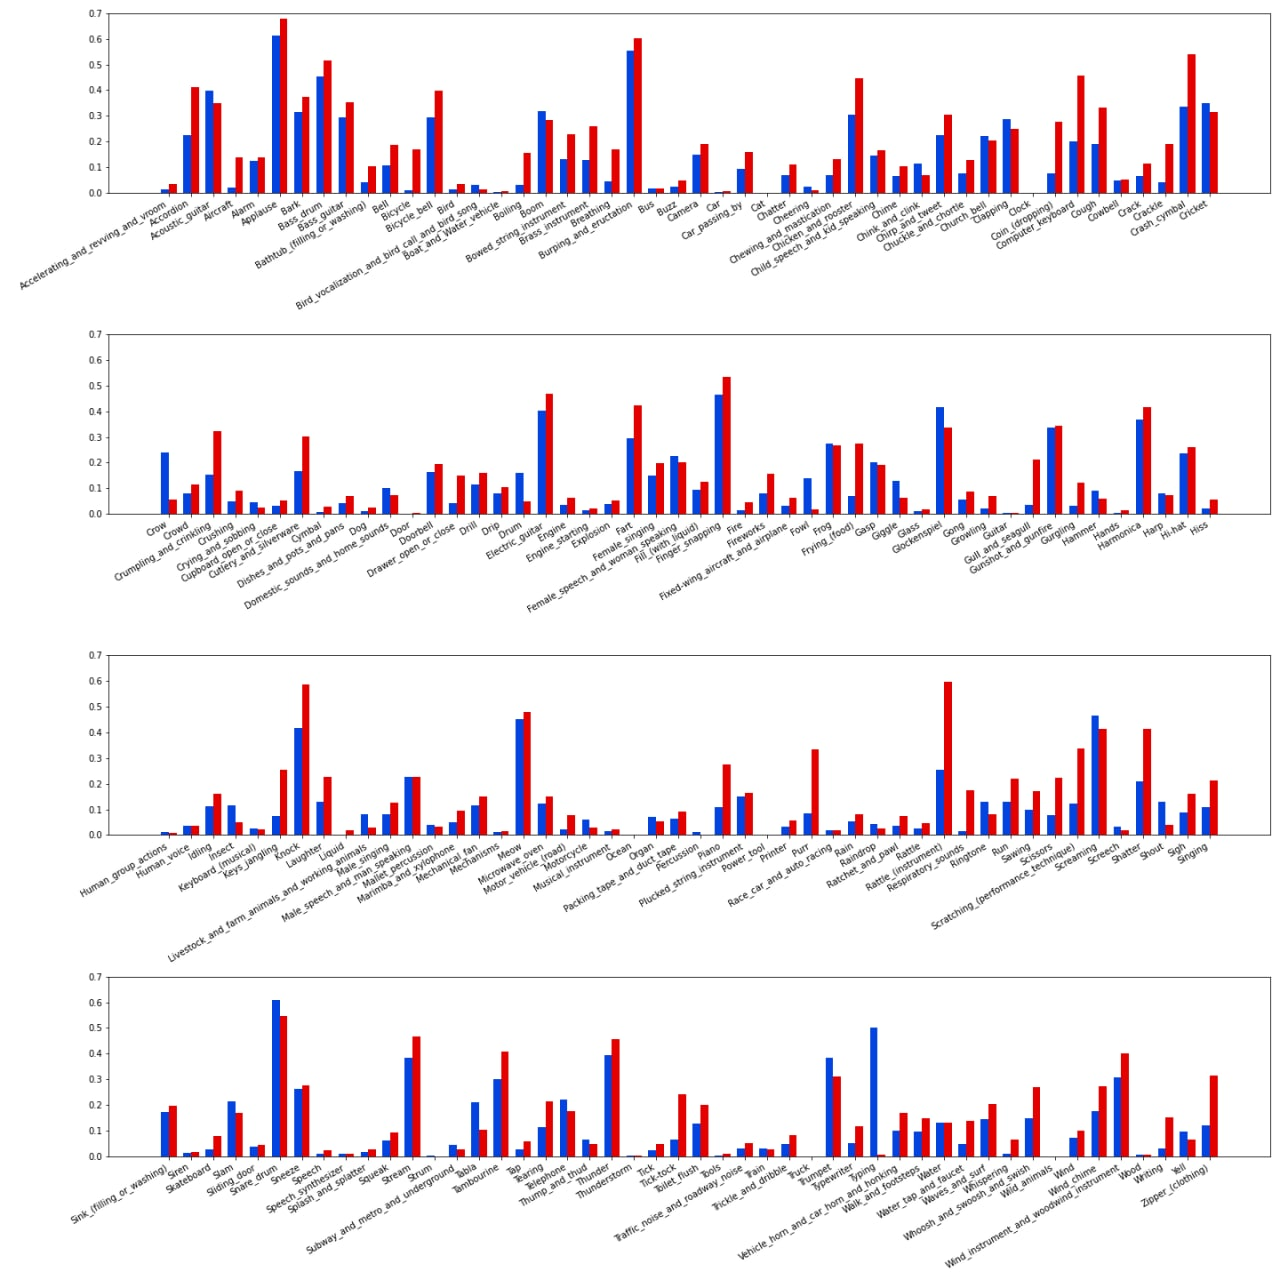
\includegraphics[width=0.49\linewidth]{assets/AP.jpg}
	\caption{Precision scores per each class. Blue bars for complex-valued network, red bars for real-valued network}
	\label{fig:apperclass}
\end{figure}


\section{Conclution}

% \begin{table}
% 	\caption{Sample table title}
% 	\centering
% 	\begin{tabular}{lll}
% 		\toprule
% 		\multicolumn{2}{c}{Part}                   \\
% 		\cmidrule(r){1-2}
% 		Name     & Description     & Size ($\mu$m) \\
% 		\midrule
% 		Dendrite & Input terminal  & $\sim$100     \\
% 		Axon     & Output terminal & $\sim$10      \\
% 		Soma     & Cell body       & up to $10^6$  \\
% 		\bottomrule
% 	\end{tabular}
% 	\label{tab:table}
% \end{table}


\bibliographystyle{unsrtnat}
\bibliography{bibliography}  %%% Uncomment this line and comment out the ``thebibliography'' section below to use the external .bib file (using bibtex) .


\end{document}